\documentclass[,table,dvipsnames]{article}
\usepackage{amsmath}
\usepackage[usenames, dvipsnames]{color}
\usepackage{graphicx}
\usepackage{caption}
\usepackage{subcaption}
\usepackage{hyperref}
\usepackage{longtable}
\usepackage{float}

\usepackage{tikz}
\usetikzlibrary{positioning}
\usetikzlibrary{shapes.geometric, arrows}
\tikzstyle{startstop} = [rectangle, rounded corners, minimum width=3cm, minimum height=1cm,text centered, draw=black, fill=red!10]
\tikzstyle{io} = [trapezium, trapezium left angle=70, trapezium right angle=110, minimum width=3cm, minimum height=1cm, text centered, draw=black, fill=blue!10]
\tikzstyle{process} = [rectangle, minimum width=3cm, minimum height=1cm, text centered, draw=black, fill=orange!10]
\tikzstyle{decision} = [diamond, minimum width=3cm, minimum height=1cm, text centered, draw=black, fill=green!10]
\tikzstyle{arrow} = [thick,->,>=stealth]

\hypersetup{
	citecolor=black,
	filecolor=black,
	linkcolor=black,
	urlcolor=black
}
\usepackage{xcolor}

\graphicspath{ {images/} {images/mat60_1AG/} }
\title{3D learning notes}
\author{xyz}
\date{Feb 2018}

\definecolor{maroon}{cmyk}{0,0.87,0.68,0.32}

\begin{document}
\noindent
\begin{titlepage}
\maketitle
\end{titlepage}	

\tableofcontents{}
\section{Deep 3D Learning Notes}

\subsection{Questions and potential improvements}
\subsubsection{potential solutions for over fitting}
\begin{itemize}
	\item combine auxiliary tasks:\par 
	1. use nxnynz as auxiliary loss
	2. boundary \par 
	3. planet \par 
	\item data augmentation: rotation, different size scale
	\item data regulation: group norm
	\item dropout
	\item combine ShapeNet data
	\item more powerful network to learn more systematic information:\par
	1. use large global block size\par
	2. dynamic sampling
	\item smaller net
\end{itemize}

\subsubsection{Important improvements}
\begin{itemize}
	\item Generate bxmh5 online. So the randomly missing part in each epoch is different. This maybe solve the info missing problem for sparse voxel 3d cnn, especially considering that block merging cannot be applied for voxel cnn. However, on line sampling can only solve missing problom of training, test missing still need some tricks to perform block merging.
	\item Check this: my usage of tf.gather\_nd should cost a lot of memory, maybe too much!
\end{itemize}


\section{Sampling and grouping}
\subsection{on line sampling and grouping progress}

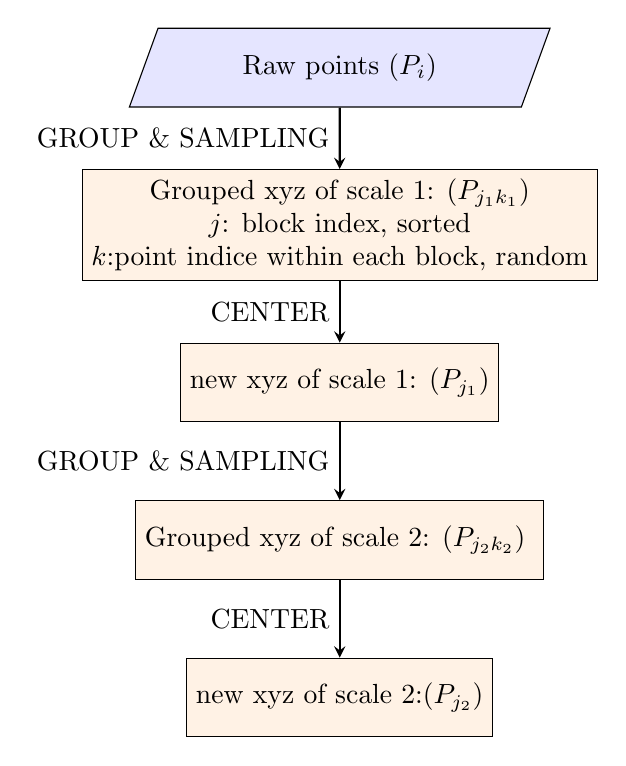
\begin{tikzpicture}[node distance=2cm]
\node (RawPoint) [io] {Raw points $(P_i)$};
\node (Grouped1) [process, below of=RawPoint, align=center] {Grouped xyz of scale 1: $({P_{j_1k_1}})$ \\ $j$: block index, sorted \\ $k$:point indice within each block, random};
\draw [arrow]  (RawPoint) -- node[anchor=east]{GROUP \& SAMPLING} (Grouped1) ;

\node (New1) [process, below of=Grouped1] {new xyz of scale 1: $({P_{j_1}})$};
\draw [arrow]  (Grouped1) -- node[anchor=east]{CENTER} (New1) ;

\node (Grouped2) [process, below of=New1, align=center] {Grouped xyz of scale 2: $({P_{j_2k_2}})$ };
\node (New2) [process, below of=Grouped2] {new xyz of scale 2:$({P_{j_2}})$};
\draw [arrow]  (New1) -- node[anchor=east]{GROUP \& SAMPLING} (Grouped2) ;
\draw [arrow]  (Grouped2) -- node[anchor=east]{CENTER} (New2) ;
\end{tikzpicture}

\subsection{GROUP}
\subsubsection{point in block}
From $(P_i)$ to $({P_{jk}})$: k is random, only need to get block index j. j solutions indicate all the blocks contain point $(P_i)$.
\par
Set parameters of block j as: 
$$ w: width $$ 
$$ s: stride $$
$$ n: point\ number\ per\ block $$
Note: do not need a parameter of padding. The containing relation should always be absolutely containing. The padding operation like CNN can be achieved just set lower limit of j.\par
The scope of block j is: $[sj,sj+w]$ \par
Let intersection point belong to right block\par
$$ sj < P_i \leq sj+w $$
$$ \frac{P_i-w}{s} \leq j < \frac{P_i}{s} $$

$$ j_L = ceil(\frac{P_i-w}{s}) $$
$$ j_U =  floor( \frac{P_i}{s})\ ( if\ \frac{P_i}{s}\ is\ float )$$\\
$$ j_U =  \frac{P_i}{s}-1\ ( if\ \frac{P_i}{s}\ is\ int )$$
$$ j:range(j_L, j_U+1) $$
To allow a bit drift of float:
$$ j_L = ceil(\frac{P_i-w}{s} - 1^{-5}) $$
$$ j_U =  floor( \frac{P_i}{s} + 1^{-5}) $$


\subsubsection{block in block}
On scale 0, the scope of block $j_0$ is: $[s_0j_0   ,s_0j_0+w_0]$ \par
On scale 1, the scope of block $j_1$ is: $[s_1j_1 ,s_1j_1+w_1]$ \par
Block $j_0$ is inside of block $j_1$.
$$ s_1j_1   <   L_0$$
$$ U_0  \leq  s_1j_1+w_1 $$

$$j_{1L}= ceil(\frac{U_0- w_1 }{s_1}-1^{-5})$$
$$j_{1U} = floor(\frac{L_0 }{s_1}+1^{-5})$$

\subsubsection{block index bound by whole raw points scope}
The scope of all points are $[P_{min}, P_{max}]$. The scope of all block index is $[j_l, j_u]$.
$$ sj_l+ padding = P_{min}$$
$$ sj_u+w-padding = P_{max} $$
$$ padding = \frac{w}{2}$$

$$ j_l = \frac{(P_{min}-padding)}{s} $$
$$ j_u = \frac{P_{max}+padding-w}{s} $$

\subsection{block indice between different scales}
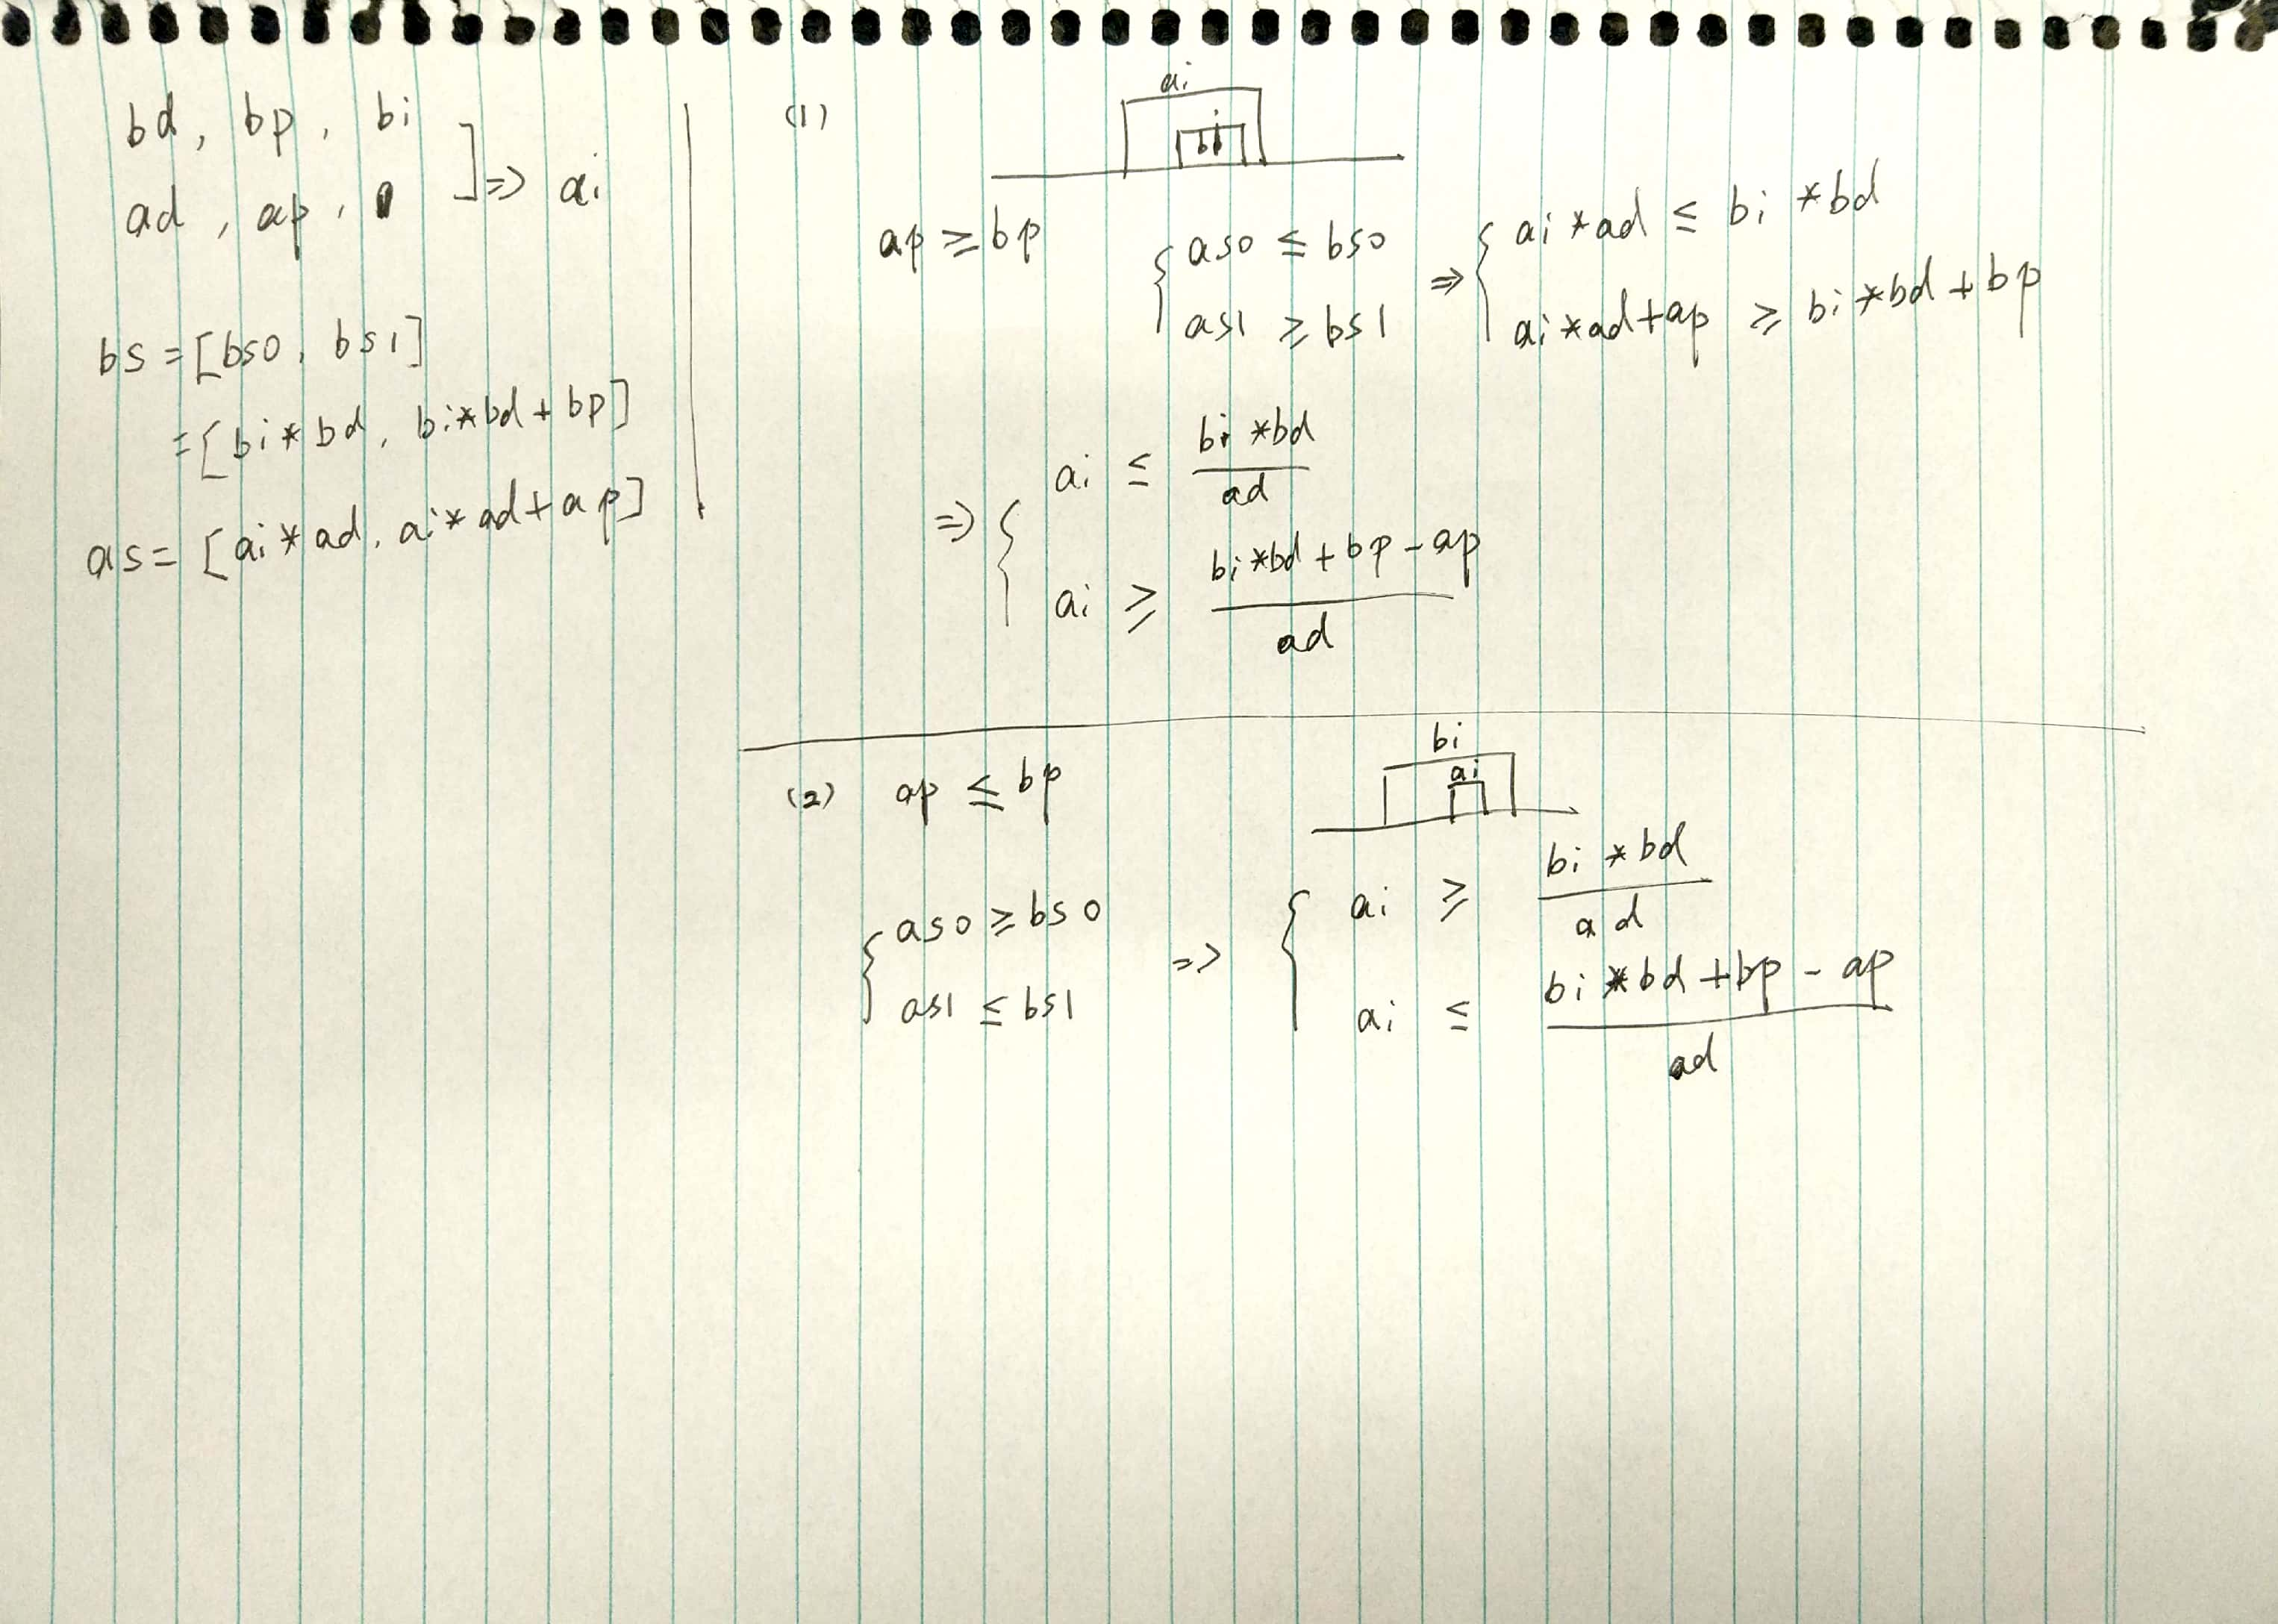
\includegraphics[width=0.9\textheight]{images_theory/bxmap.png}


\subsection{voxelizatiopn configuration}
$$ steps = [0.1,0.3,0.9,2.7] + [-6.3]$$
$$ strides = [0.1,0.2,0.6,1.8] + [-3.6] $$
$$ voxel\ size=[, 3, 4, 4, 3] $$
principles:\par
(1)Alignment between differert scales:
$$ steps[i] = steps[i-1]+strides[i-1]*(k-1)\  (k=voxel\ size) $$
(2)Alignment between voxels on one scale:
$$ strides[i] \% steps[i-1] == 0 $$
Examples:\par
$$ 0.3=0.1+0.1*2 \Rightarrow voxel\ size=3 $$
$$ 0.2=0.1*2 $$
$$ 0.9=0.3+0.2*3 \Rightarrow voxel\ size=4 $$ 
$$ 0.6=0.3*2 $$
$$$$
$$ 6.3=2.7+1.8*2 $$
$$ 3.6=1.8*2 $$

\subsection{Flatten from pidx\_bididx\_unsampled}
pidx\_bididx\_unsampled is global block augmented.

$$ start\_bid\_step=10 $$
$$ start\_pidx\_step=20 $$
$$ unique\ block\ num=7 $$
\[  
\begin{bmatrix}
pidx \\ 4 \\ 2 \\ 1 \\ 1 \\2 \\-- \\23 \\20 \\ 25\\21 \\23\\23
\end{bmatrix}
\begin{bmatrix}
bid \\ 1 \\ 1 \\ 3 \\ 5 \\ 5  \\--  \\12 \\14\\14\\17\\17\\18
\end{bmatrix}
\begin{bmatrix}
bididx \\ 0 \\ 0 \\ 1 \\ 2 \\2 \\-- \\3\\4\\4\\5\\5\\6
\end{bmatrix}
\begin{bmatrix}
valid\ bock\\ sampling\ g\_index \\\\2\\3\\4\\--\\5\\ \\ \\8\\9\\10
\end{bmatrix}
\]
\subsubsection{get valid block sampling g\_index to sampling valid blocks}
\[  
\begin{bmatrix}
unique\\ bid \\ 1\\ 3\\ 5\\ 12 \\14 \\ 17\\18
\end{bmatrix}
\begin{bmatrix}
bididx \\ \\ 0\\1\\2\\3\\4\\5\\6
\end{bmatrix}
\begin{bmatrix}
count \\ \\ 2\\ 1\\ 2\\ 1 \\2 \\ 2\\1
\end{bmatrix}
\begin{bmatrix}
cumsum\\ count \\ 2\\ 3\\ 5\\ 6 \\8 \\ 10\\11
\end{bmatrix}
~~~
\begin{bmatrix}
sampled\\ bid \\  3\\ 5\\ 12  \\ 17\\18
\end{bmatrix}
\begin{bmatrix}
sampled\\ bididx \\  1\\ 2\\ 3  \\ 5\\6
\end{bmatrix}
\begin{bmatrix}
the\\ count \\  1\\ 2\\ 1  \\ 2\\1
\end{bmatrix}
\begin{bmatrix}
the\ sum\\ count \\ 3\\ 5\\ 6 \\ 10\\11
\end{bmatrix}
\begin{bmatrix}
start\\ g\_index \\3-1=2\\5-2=3\\6-1=5 \\10-2=8\\11-1=10
\end{bmatrix}
\]

\subsubsection{get flat idx: block index for each point}
\[  
\begin{bmatrix}
pidx \\ 1 \\ 1 \\2 \\-- \\ 23\\21 \\23\\23
\end{bmatrix}
\begin{bmatrix}
bididx  \\ 1 \\ 2 \\2 \\-- \\ 3 \\ 5 \\ 5\\6
\end{bmatrix}
sort\ by\ pidx
\begin{bmatrix}
pidx \\ 1 \\ 1 \\2 \\-- \\ 21 \\  23 \\23\\23
\end{bmatrix}
\begin{bmatrix}
bididx  \\ 1 \\ 2 \\2 \\-- \\ 5 \\ 3 \\ 5\\6
\end{bmatrix}
->
\begin{bmatrix}
pidx\ same\\ with\ last  \\ 0 \\ 1 \\0 \\-- \\ 0 \\ 0 \\ 1 \\ 1
\end{bmatrix}
->
\begin{bmatrix}
psl\ cum\\sum  \\ 0 \\ 1 \\1 \\-- \\ 1 \\ 1 \\ 2 \\ 3
\end{bmatrix}
-
\begin{bmatrix}
sampled\\ piccs\\0\\0\\1\\--\\1\\1\\1\\1
\end{bmatrix}
=
\begin{bmatrix}
flat\_idx  \\ 0 \\ 1 \\0 \\-- \\ 0 \\ 0 \\ 1\\ 2
\end{bmatrix}
\]
******
\[
\begin{bmatrix}
unique\ pidx \\  1\\ 2\\21 \\23
\end{bmatrix}
\begin{bmatrix}
count \\ 2\\1\\1\\3
\end{bmatrix}
\begin{bmatrix}
count-1 \\  1\\0\\0\\2
\end{bmatrix}
\begin{bmatrix}
cumsum \\  1\\1\\1\\3
\end{bmatrix}
\begin{bmatrix}
piccs \\  0\\1\\ 1\\1
\end{bmatrix}
->
\begin{bmatrix}
pidxidx\\0\\0\\1\\--\\2\\3\\3\\3
\end{bmatrix}
\begin{bmatrix}
sampled\ piccs\\0\\0\\1\\--\\1\\1\\1\\1
\end{bmatrix}
\]


\subsection{Flatten from grouped point index}
The disadvantage for this solution: cannot get the flat idx for abandoned points.
$$ 5 => grouped\ point\ index => (2,4) $$
\[ grouped\ point\ index =  \begin{bmatrix}
2 & 3 & 4 & -1 \\ 0 & 2 & 3 & -1
\end{bmatrix} \]
\subsubsection{A}
\[  
\begin{bmatrix}
2 & 0 \\ 3 & 0 \\  4 & 0 \\ -1 & 0 \\ 0 & 1\\ 2 & 1\\ 3 & 1 \\ -1 & 1
\end{bmatrix} 
\begin{bmatrix}
2 & 0 \\ 3 & 0 \\  4 & 0 \\ 0 & 1\\ 2 & 1\\ 3 & 1 
\end{bmatrix} 
\begin{bmatrix}
0 & 1 \\ 2 & 0 \\  2 & 1 \\ 3 & 0\\ 3 & 1\\ 4 & 0 
\end{bmatrix} 
gp\ same\ with\ last
\begin{bmatrix}
0 \\ 0 \\ 1 \\ 0 \\ 1 \\ 0 
\end{bmatrix} 
cumsum
\begin{bmatrix}
0 \\ 0 \\ 1 \\ 1 \\ 2 \\ 2 
\end{bmatrix} 
\]

\subsubsection{B}
\[  
\begin{bmatrix}
0 \\ 2 \\ 2 \\ 3 \\3 \\ 4 
\end{bmatrix}
unique
\begin{bmatrix}
0 \\ 2 \\ 3 \\ 4 
\end{bmatrix} 
count
\begin{bmatrix}
1 \\ 2 \\ 2 \\ 1
\end{bmatrix} 
-1=
\begin{bmatrix}
0 \\ 1 \\ 1 \\ 0
\end{bmatrix}
cum\ sum
\begin{bmatrix}
0 \\ 1 \\ 2 \\ 2
\end{bmatrix}
cat\ 0\ at\ begining
\begin{bmatrix}
0\\ 0 \\ 1 \\ 2 \\ 2
\end{bmatrix}
\]

\subsubsection{C}
\[  unique\ idx
\begin{bmatrix}
0 \\ 1 \\ 1 \\ 2 \\ 2 \\3 
\end{bmatrix}
the\ cum\ sum
\begin{bmatrix}
0 \\ 0 \\ 0 \\ 1 \\ 1 \\2 
\end{bmatrix}
\]

\[ 
\begin{bmatrix}
0 \\ 0 \\ 1 \\ 1 \\ 2 \\ 2 
\end{bmatrix}
-
\begin{bmatrix}
0 \\ 0 \\ 0 \\ 1 \\ 1 \\2 
\end{bmatrix}
=
\begin{bmatrix}
0 \\ 0 \\ 1 \\ 0 \\ 1 \\0
\end{bmatrix}
\]

\subsubsection{D}
\[ 
\begin{bmatrix}
gp & block\_id & flat\_id
\end{bmatrix}
=
\begin{bmatrix}
	0 & 1 \\ 2 & 0 \\  2 & 1 \\ 3 & 0\\ 3 & 1\\ 4 & 0 
\end{bmatrix} 
\begin{bmatrix}
0 \\ 0 \\ 1 \\ 0 \\ 1 \\0
\end{bmatrix}
\]

\subsubsection{E}
scatter\_nd(indices=[gp,flat\_id], \par updates=block\_id, shape=(num\_point\_last\_scale, flatten\_num))



\section{Data Augmentation} 
\begin{itemize}
\item (1.1) Rotate corrdinate reference: Rotate both point and voxel box \par
Performed by rotating points after sampling and grouping. \par
This should only be applied to point position (cascade 0). What if also to features (upper cascades).

\item (1.2) Rotae point only, or rotate voxel box only. \par
a) It can be performed by rotating points before sampling and grouping.\par
b) If rotate angle is integral times of pi/2, it can be performed by rotating point indices inside the voxel.\par
Rotate voxel can be applied to all cascades.
\item (2.1) Rotate the global block by the same angle
\item (2.2) Rotate each voxel by seperate angle in each scale.\par
Since the features are calculated independently in each voxel, it should be fine to apply different rotatio angle for each voxel. It doesn't matter that the rotation center is voxel center or global block center. It alos doesn't matter that it rotates refference or only rotates voxel.

\end{itemize}

\section{Sparse voxel 3DCNN }
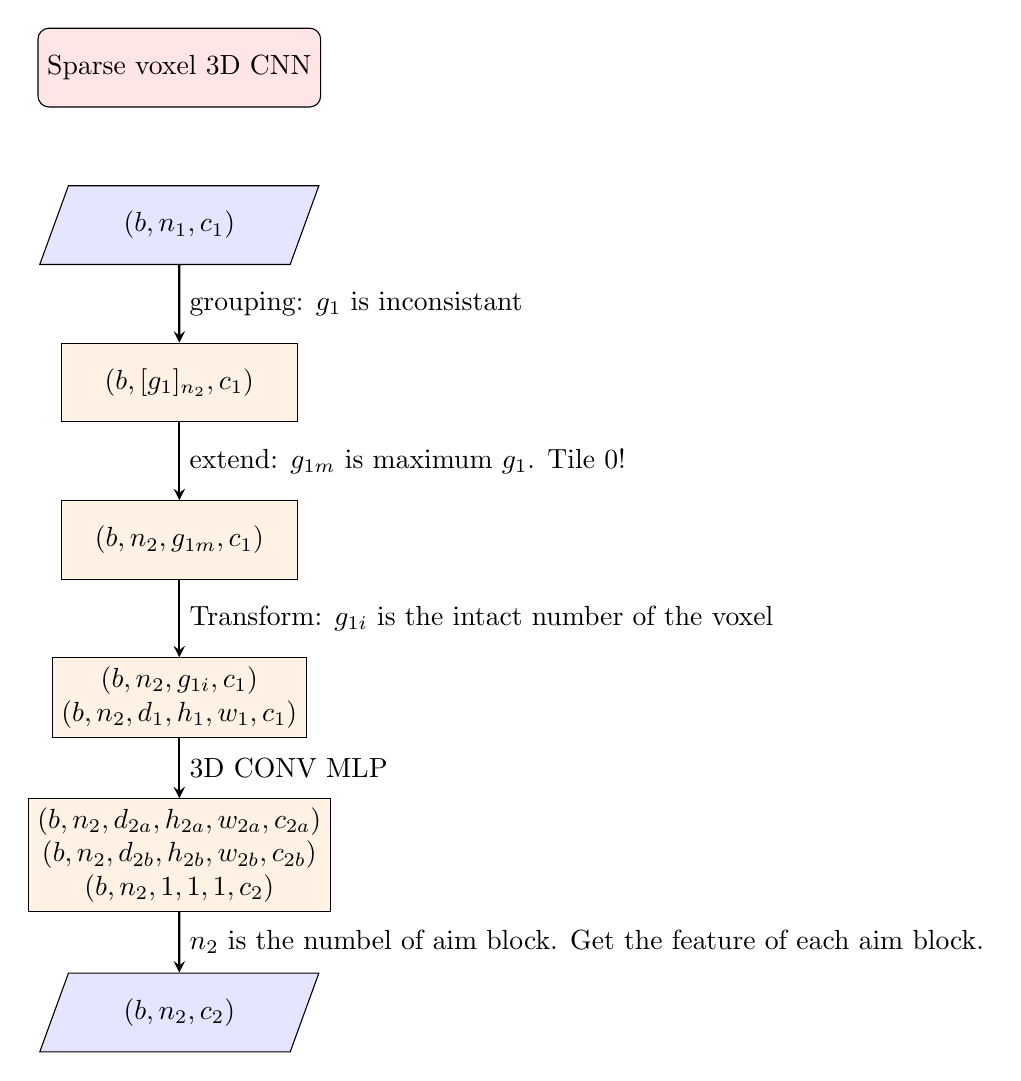
\begin{tikzpicture}[node distance=2cm]
	\node (start) [startstop] {Sparse voxel 3D CNN};
	\node (in) [io, below of=start] {$(b,n_1,c_1)$};
	\node (group) [process, below of=in] {$(b,[g_1]_{n_2},c_1)$};
	\draw [arrow] (in) -- node [anchor=west] {grouping: $g_1$ is inconsistant} (group);
	\node (extend) [process, below of=group] {$(b,n_2,g_{1m},c_1)$};
	\draw [arrow] (group) -- node [anchor=west] {extend: $g_{1m}$ is maximum $g_1$. Tile 0!} (extend);
	\node (transform) [process, below of=extend, align=center] {$(b,n_2,g_{1i},c_1)$ \\ $(b,n_2,d_1,h_1,w_1,c_1)$};
	\draw [arrow] (extend) -- node [anchor=west] {Transform: $g_{1i}$ is the intact number of the voxel} (transform);
	\node (3dconv) [process, below of=transform, align=center] {$(b,n_2,d_{2a},h_{2a},w_{2a},c_{2a})$\\ $(b,n_2,d_{2b},h_{2b},w_{2b},c_{2b})$ \\$(b,n_2,1,1,1,c_2)$};
	\draw [arrow] (transform) -- node [anchor=west] {3D CONV MLP} (3dconv);
	\node (out) [io, below of=3dconv] {$(b,n_2,c_2)$};
	\draw [arrow] (3dconv) -- node [anchor=west] {$n_2$ is the numbel of aim block. Get the feature of each aim block.} (out);
\end{tikzpicture}
\par \par
Two main obstacles for performing 3D convolution on point cloud are: (1) there are too many vacant points, (2) the position of points are not aligned.
The key idea of sparse voxel is to perform 3DCONV on cascades from the second. Because the positions are actually almost aligned. At the same time, the vacant rate within a small block is acceptably large. Above all, it may be possible to do apply 3D-CONV within a small block. 
\par
Centres of blocks in cascades other than first one are actually aligned to the grid. So it is possible to perform 3d convolution directly. However, the average position of points inside these blocks are not aligned. Thus it is also maybe beneficial to utilise a transform net to align them.\par
On the other hand, there are many vacant points in the block. I am wondering if it is beneficial to set the features of vacant points by a T-net from around existing points.
\par

Purpose of T-Net: fix number + align + till \par
There are some interesting problems for Transform net:
\begin{itemize}
	\item Only depend on position or feature.
	\item Should be resolution invariant.
	\item If it should be constant for all channels.
	\item If it should be constant for all local aim blocks.
\end{itemize}
\par
Reasons that we do not need the T-Net:
\begin{itemize}
	\item 3d-conv can till features of the vacant points.
	\item If the base-points are not strictly aligned, add the position to feature map. Or get a special feature of positions within the block and then add ot the main feature map.
\end{itemize}
\par
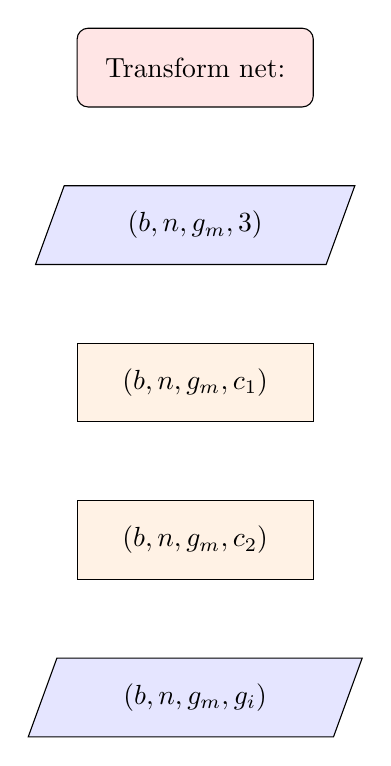
\begin{tikzpicture}[node distance=2cm]
	\node (start) [startstop] {Transform net: };
	\node (in) [io, below of=start] {$(b,n,g_m,3)$};
	\node (p1) [process, below of=in] {$(b,n,g_m,c_1)$};
	\node (p2) [process, below of=p1] {$(b,n,g_m,c_2)$};
	\node (out) [io, below of=p2] {$(b,n,g_m,g_i)$};
\end{tikzpicture}

\newpage
\section{Graph neural network for high resolution indoor mesh}
Items need to reconsider
\begin{itemize}
	\item Down sample by points or faces
	\item How to add new edges after down-sampling
	\item Design the best operation for dynamic graph that may be highly unbalance. Is it still ok to share weights for each edges. If not, how to differentiate.
	\item What if not enough edges available
\end{itemize}

\par \noindent
Key ideas:
\begin{itemize}
	\item Indoor meshes are mostly planar and simple faces. Semantically down sample the mesh and remove the simple faces.
	\item Novel graph CNN to better capture features for highly unbalanced mesh 
	\item Make use of raw resolution
	\item Handle large scale point clouds
	\item Make best use of mesh graph when searching local structure
\end{itemize}

\subsection{basic framework}
\usetikzlibrary{positioning}
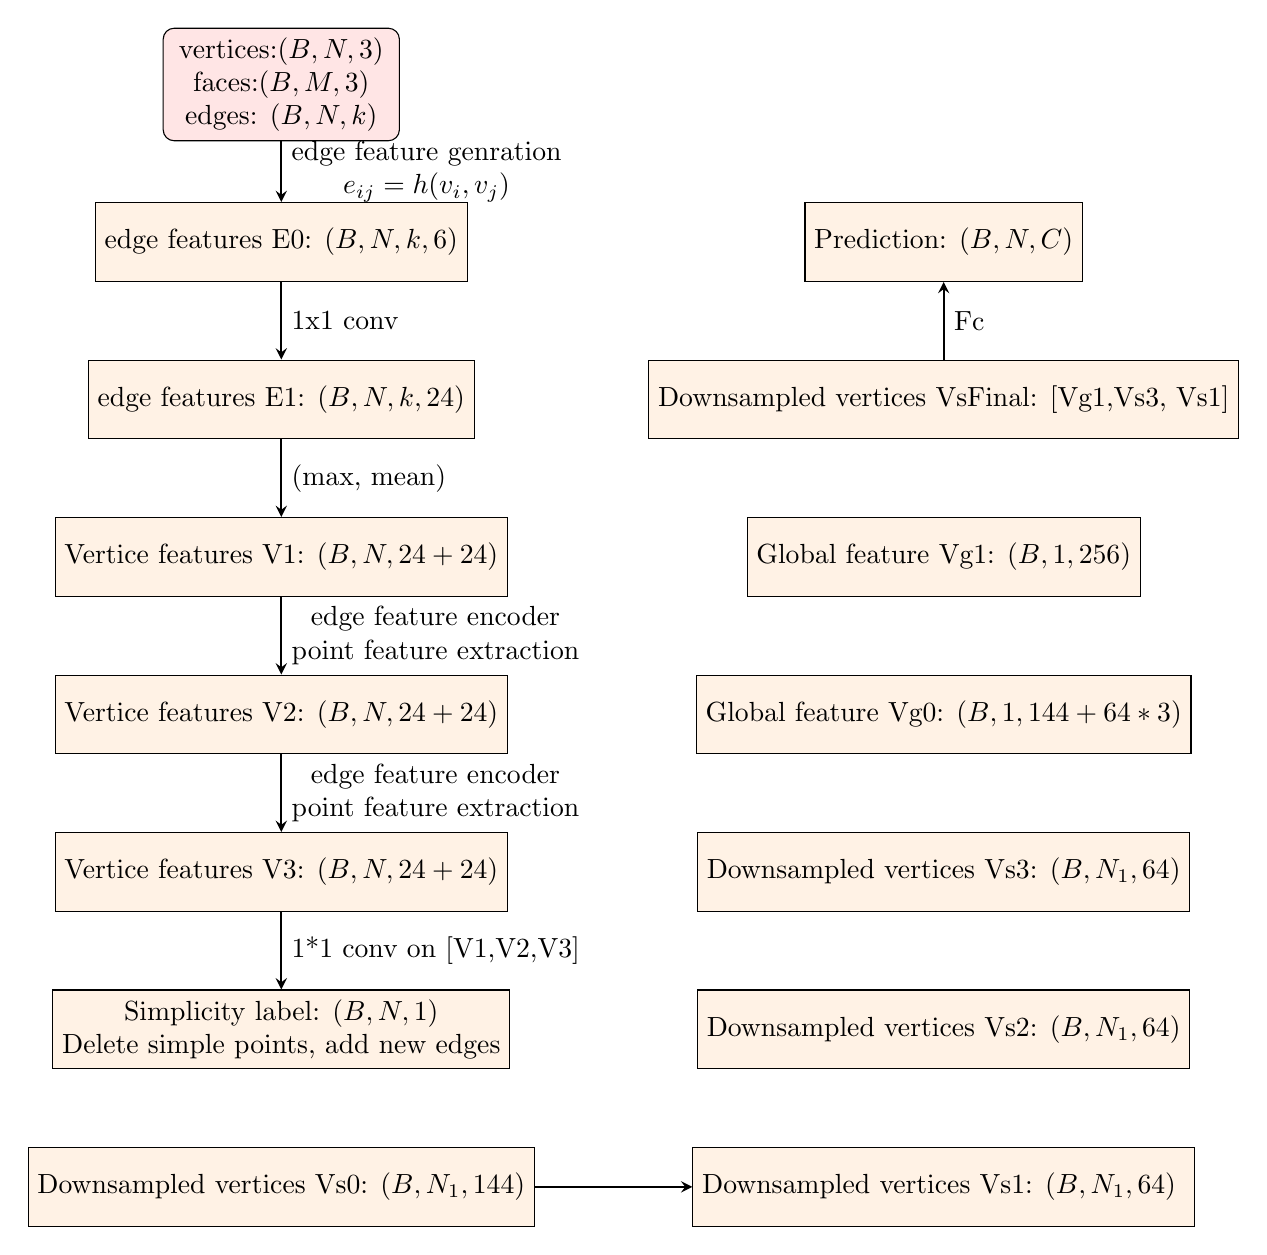
\begin{tikzpicture}[align=center, node distance=2cm]
\node (start) [startstop] 
{vertices:$(B,N,3)$ \\ faces:$(B,M,3)$ \\ edges: $(B,N,k)$};

\node (p1) [process, below of=start] 
{edge features E0: $(B,N,k,6)$};
\draw [arrow] (start) -- node [anchor=west] {edge feature genration \\ $e_{ij} = h(v_i, v_j)$} (p1);

\node (p2) [process, below of=p1] 
{edge features E1: $(B,N,k,24)$};
\draw [arrow] (p1) -- node [anchor=west] {1x1 conv} (p2);

\node (p3) [process, below of=p2,] 
{Vertice features V1: $(B,N,24+24)$};
\draw [arrow] (p2) -- node [anchor=west] {(max, mean)} (p3);

\node (p4) [process, below of=p3] 
{Vertice features V2: $(B,N,24+24)$};
\draw [arrow] (p3) -- node [anchor=west] {edge feature encoder \\ point feature extraction} (p4);

\node (p5) [process, below of=p4] 
{Vertice features V3: $(B,N,24+24)$};
\draw [arrow] (p4) -- node [anchor=west] {edge feature encoder \\ point feature extraction} (p5);

\node (p6) [process, below of=p5] 
{Simplicity label: $(B,N,1)$ \\Delete simple points, add new edges};
\draw [arrow] (p5) -- node [anchor=west] {1*1 conv on [V1,V2,V3]} (p6);

\node (Vs0) [process, below of=p6] 
{Downsampled vertices Vs0: $(B,N_1,144)$};

\node (Vs1) [process, right=2cm of Vs0 ]
{Downsampled vertices Vs1: $(B,N_1,64)$ };
\draw [arrow] (Vs0) -- node [anchor=west] {} (Vs1);

\node (Vs2) [process, above of=Vs1 ] 
{Downsampled vertices Vs2: $(B,N_1,64)$};

\node (Vs3) [process, above of=Vs2 ] 
{Downsampled vertices Vs3: $(B,N_1,64)$};

\node (Vg0) [process, above of=Vs3 ] 
{Global feature Vg0: $(B,1,144+64*3)$};

\node (Vg1) [process, above of=Vg0 ] 
{Global feature Vg1: $(B,1,256)$};

\node (Vsf) [process, above of=Vg1 ] 
{Downsampled vertices VsFinal: [Vg1,Vs3, Vs1]};

\node (L) [process, above of=Vsf ] 
{Prediction: $(B,N,C)$};
\draw [arrow] (Vsf) -- node [anchor=west] {Fc} (L);

\end{tikzpicture}

\subsubsection{Point cloud triangulation}
matterport dataset
\subsubsection{point feature encoder}
Enocode low level point features based on graph cnn.
\subsubsection{predict simple points}
\begin{itemize}
	\item it's planar 2 edges around
	\item it's all belong to the same category 2 edges around
\end{itemize}
planar points not at the edge of an object
\subsubsection{delete simple points and add new edges}

Generate the down sampled ground truth at the same time. If the new face contains different semantics, which is incorrect, set as fail label.
\par \noindent
The target:
\begin{itemize}
	\item Significantly reduce resolution: to 10\%
	\item Do not lost shape information
	\item Do not lost semantic information
	

	
\end{itemize}
\subsubsection{learn higher level features on new point cloud}
The mesh graph can be highly unbalanced. The weight for each edge may not be shared directly. 

\subsection{point representation or face representation}
\subsubsection{point representation}
Operation:
$$f_i^{l+1} = W_0f_i^l + \sum_{j\in N(i)}W_1 f_j^l$$
$$f_i^{l+1} = W_0f_i^l + max_{j\in N(i)}W_1 f_j^l$$
$$f_i^{l+1} = \sum_{j\in N(i)}W(x_i, x_j-x_i) $$
$$f_i^{l+1} = \max_{j\in N(i)}W(x_i, x_j-x_i) $$
\par \noindent

\begin{itemize}
	\item raw data format from sensors
	\item search for neighbour points
	\item the number of points are smaller than edges and faces
\end{itemize}

\subsubsection{face representation}
Operation:
$$f^0 = max\{x_0, x_1, x_2\}$$
$$f_i^{l+1} = W_0f_i^l + \sum_{j\in N(i)}W_1 f_j^l$$
\par \noindent

\begin{itemize}
	\item Better real meaning for labels. Commonly used for 3D viewers. Used in Matterport Dataset.
	\item Search for neighbour faces
	\item Still have to get point feature at first
\end{itemize}

\subsubsection{solution 1}
Use point representation during feature extraction and down-sampling. Choose to predict point label or face label at last. 

\subsubsection{edge feature genration}



\section{KNN acceleration}

\end{document}